\newpage
\noindent
\textbf{Beispiel 2}\\ \\
Wärmeübergänge werden als Widerstände, Bereiche mit veränderlicher Temperatur als Kapazitäten, konstante Temperaturen als Spannungsquellen und zugeführte Leistungen als Stromquellen dargestellt. Daher ergibt sich für die RC-Ersatzschaltung dieses Problems
\begin{figure}[h]
	\centering
	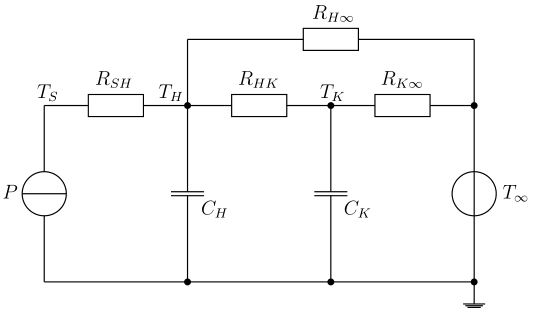
\includegraphics[width= 10cm]{tikz/27_09_2019_2a}
\end{figure}
Aus dieser Ersatzschaltung folgen die Differentialgleichungen
\begin{align*}
	C_H\dot{T}_H &= P - \frac{1}{R_{H\infty}}(T_H - T_\infty) - \frac{1}{R_{HK}(T_H - T_K)} \\
	C_K\dot{T}_K &= -\frac{1}{R_{K\infty}}(T_K - T_\infty) + \frac{1}{R_{HK}(T_H - T_K)}
\end{align*}
Diese Gleichungen können analog wie bei elektrischen Netzwerk bestimmt werden. Hier sind die \textit{Spannungen} Temperaturen und die \textit{elektrischen Ströme} Wärmeströme bzw. Leistungen.\\ \\
b)\\ \\
Über den Gesamten thermischen Widerstand
\[
	R_{ges} = \frac{R_{H\infty}(R_{HK} + R_{K\infty})}{R_{H\infty} + R_{H\infty}(R_{HK} + R_{K\infty}} + R_{SH}
\]
und der geforderten Bedingung aus der Angabe folgt
\[
	2T_\infty = R_{ges}P
\]
Damit folgt für den gesuchten thermischen Widerstand
\[
	R_{SH} = \frac{2T_\infty}{P} - \frac{R_{H\infty}(R_{HK} + R_{K\infty})}{R_{H\infty} + R_{H\infty}(R_{HK} + R_{K\infty}}
\]
\newpage
\noindent
c)\\ \\
Mit $\tau = R_\infty(C_H + C_K)$ und $R_\infty = \frac{R_{H\infty}R_{K\infty}}{R_{H\infty}+R_{K\infty}}$ und den obigen Gleichungen und den gegebenen Anfangstemperaturen folgt den gesuchten Temperaturverlauf
\[
	T_S(t) = R_{SH}P + (T_0 - R_\infty P - T_\infty)e^{-\frac{t}{\tau}} + R_{\infty}P + T_\infty
\]
d)\\ \\
Mit dem veränderten $\tau = R_{H\infty}C_H$ folgt für den neuen Temperaturverlauf unter Berücksichtigung von $t_{crit}$ und $T_{crit}$
\[
	T_S(t) = R_{SH}P + (T_{crit} - R_{H\infty} P - T_\infty)e^{\frac{-(t - t_{crit})}{\tau}} + R_{H\infty}P + T_\infty
\]
und somit lautet die maximale Temperatur für den Schaltkreis
\[
	T_{S,max} = (R_{SH} + R_{H\infty})P + T_\infty
\]
\textit{Hinweis : Ersichtlich aus der Ersatzschaltung} \\ \\